
\chapter{Custom Templates}
\label{template}

In the "Database" -> "Open template editor" menu you can configure custom labels, bit
mappings and any integer/float/string conversions to be associated with the various registers.

\begin{figure}[H]
    \centering
    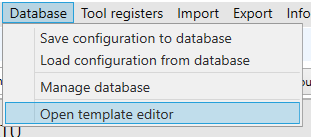
\includegraphics[width=0.4\textwidth]{../Img/Menu_Database.PNG}
    \caption{Database menu}
\end{figure}

The window for entering custom templates associated with the various registers is as follows:

\begin{figure}[H]
\centering
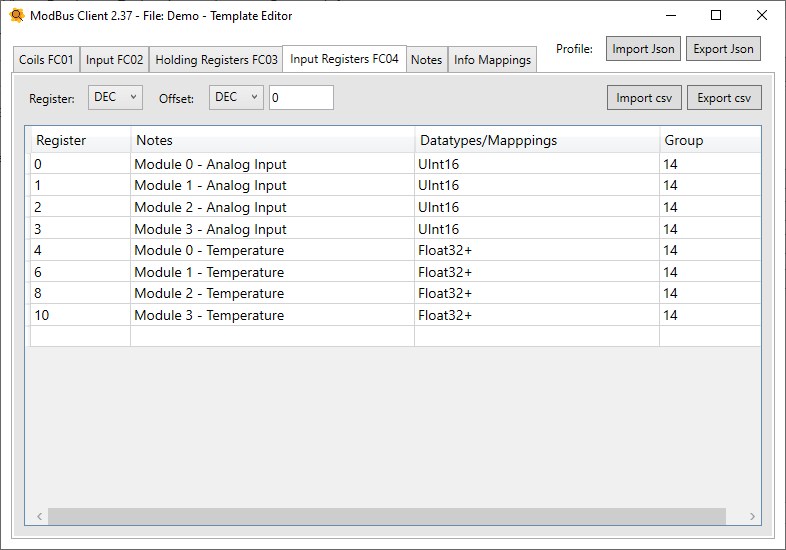
\includegraphics[width=0.80\textwidth]{../Img/ModBus_Client_Template_00.PNG}
\caption{Template editor}
\end{figure}

For each register in the template window you associate a possible label, the corresponding datatype,
and whether you want one or more resource groups to which the current group should be added.
For each register you can specify whether the value is entered in 
decimal or hexadecimal and also you can add an offset 
to the registers. In the same window you can specify whether the registers entered
are to be considered in decimal or hexadecimal and a possible offset (positive or negative)
to be added to the values entered.
For example, an offset of 100 moves the label of register 10 to the
position 110. This is convenient if, for example, a PLC has the \%MW0 starting at offset
0x4000. In this case you fill in the table starting at 0 and then simply set as the
offset the value HEX 4000.

In the case where different models of PLCs have different position
of the \%MW, to switch from one model to another is
simply change the offset without having to go and change the registers 
one by one
(negative offsets can also be applied
should it be necessary).
Following are screenshots of some examples based on the template
of the previous image:

\begin{figure}[H]
\centering
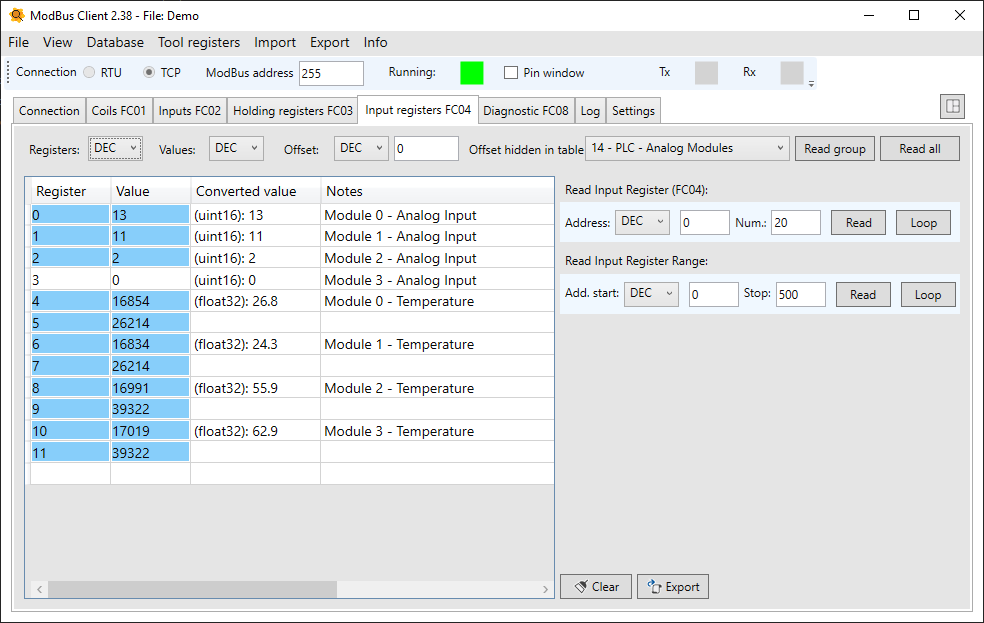
\includegraphics[width=0.70\textwidth]{../Img/ModBus_Client_Template_ReadDemo00.PNG}
\caption{Template editor}
\end{figure}

The "Notes" column displays the descriptions of the various registers 
while the "Converted Value" column displays the contents
of each register converted to the assigned datatype. In this way it is very simple to 
convert 32- or 64-bit values, floats or strings to the actual value.
By selecting a group from the drop-down menu also the client goes to read the registers
of the selected group in ascending order.

In the template window you can define multiple resource groups and
associate them with the various registers, so in the main window you can 
you can read different registers (even non-consecutive ones)
by calling up the corresponding resource group.

\begin{figure}[H]
\centering
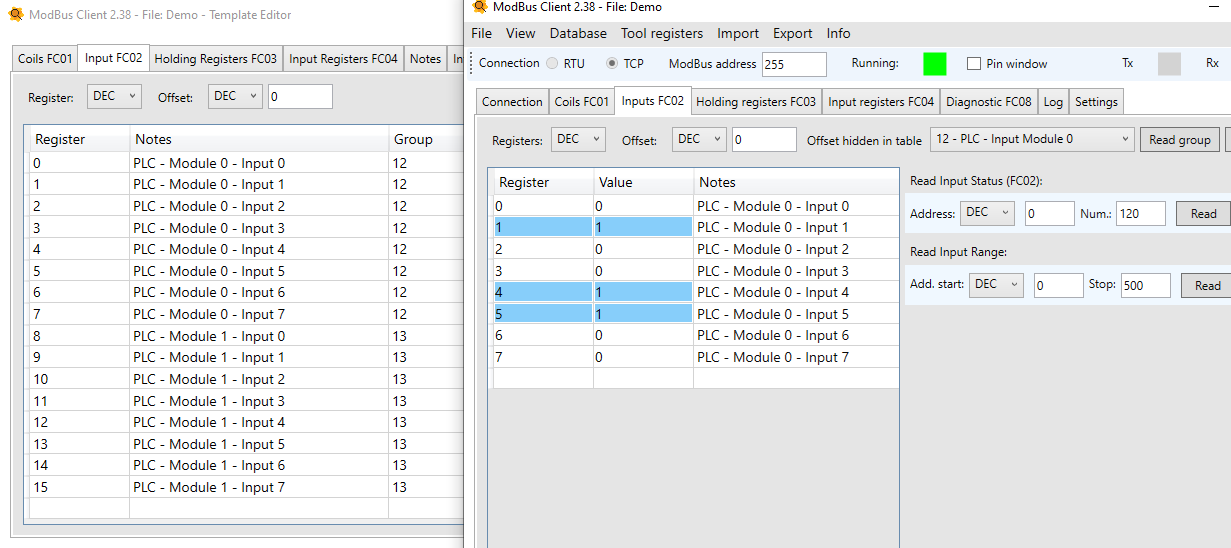
\includegraphics[width=0.85\textwidth]{../Img/ModBus_Client_Template_Group00.PNG}
\caption{Group resources}
\end{figure}

\section{Group definition}

In the "Notes" tab of the template window, it is possible to define resource groups
to be called up later in the main window. It is not necessary to enter the groups in order.

\begin{figure}[H]
\centering
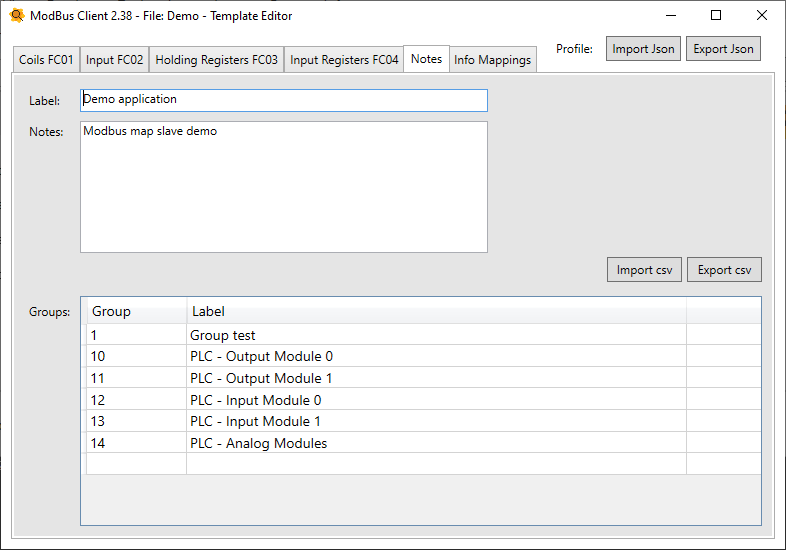
\includegraphics[width=0.70\textwidth]{../Img/ModBus_Client_Template_Group_Definition.PNG}
\caption{Group definition}
\end{figure}

The last tab "Info Mappings" contains a summary of the datatypes implemented and managed by the client.

\begin{figure}[H]
\centering
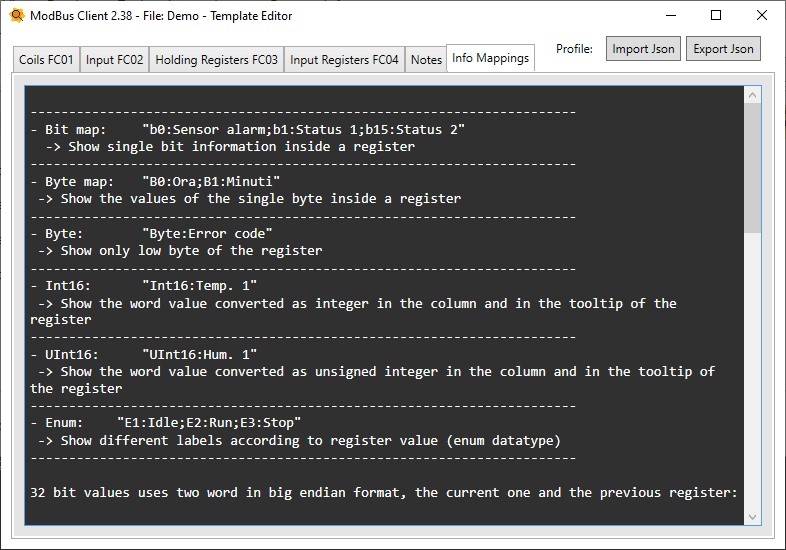
\includegraphics[width=0.70\textwidth]{../Img/ModBus_Client_Template_Info_Mappings.PNG}
\caption{Mappings info}
\end{figure}

\newpage
\section{Datatypes}

The following are the various datatypes supported by the program and configurable in a profile template.

\subsubsection{Bit map}

It shows the individual bits of the word in the line tooltip with the resource label next to it.

\begin{verbatim}
    b0:230v presence;b1:Status 1;b15:Status 2
\end{verbatim}

\subsubsection{Byte map}

It shows the two bytes of the word.

\begin{verbatim}
    B0:Hour;B1:Minutes
\end{verbatim}

\subsubsection{Int16 / UInt16}

It shows the word as a signed integer.

\begin{verbatim}
    Int16:Temp. 1
    UInt16:Counter
\end{verbatim}

The following 32-bit (two word) variables use the previous (High Word) and
current (Low Word) referenced in the Big Endian format.

\subsubsection{Float}

It collects two words and displays the data in float in the row tooltip.

\begin{verbatim}
    Float:Temperatura locale 1
\end{verbatim}

\subsubsection{Int32 / UInt32}

It collects two words and displays the data in int32 or uint32 in the line tooltip.

\begin{verbatim}
    Int32:Temperatura locale 1
    UInt32:Temperatura locale 2
\end{verbatim}

The following 64-bit variables (two words) use the three words of the previous (High Word) and
current (Low Word) referenced in the Big Endian format. With the modifiers 
format you can specify whether to use the current register and the next three.
\subsubsection{Int64 / UInt64}

\begin{verbatim}
    Int64:Timestamp start time
    UInt64:Timestamp start time
\end{verbatim}

\subsubsection{String(len[, offset])}

With string objects, it is possible to convert the contents of registers
to string (NULL terminated string). In the example below
8 bytes are converted into 8 ASCII characters with an offset of -2
(the string starts at the previous register).

\begin{verbatim}
    String(8,-2):Model
\end{verbatim}

\section{Datatype modifiers}

\subsubsection{Swap}

Adding a dash "-" or "\_swap" string multiple words
values are converted in little endian format.

\begin{verbatim}
    Swap: "UInt32-" "UInt32_swap"
\end{verbatim}

\subsubsection{Word offset}

Adding a plus sign "+" multiple words values 
uses the current register and the next ones to cast the content.

\begin{verbatim}
    Offset: "UInt32+"
\end{verbatim}

\subsubsection{Word offset + Swap}

\begin{verbatim}
    "UInt32-+" oppure "UInt32_swap+"
\end{verbatim}

Combine the previous two, use the current and next register in the Little Endian format.

\newpage

The following screenshots contains some examples
of different templates.
\\\\
Template:

\begin{figure}[H]
\centering
\includegraphics[width=0.75\textwidth]{../Img/Modbus_Client_Template_00.PNG}
\caption{}
\end{figure}

Example of final conversion:

\begin{figure}[H]
\centering
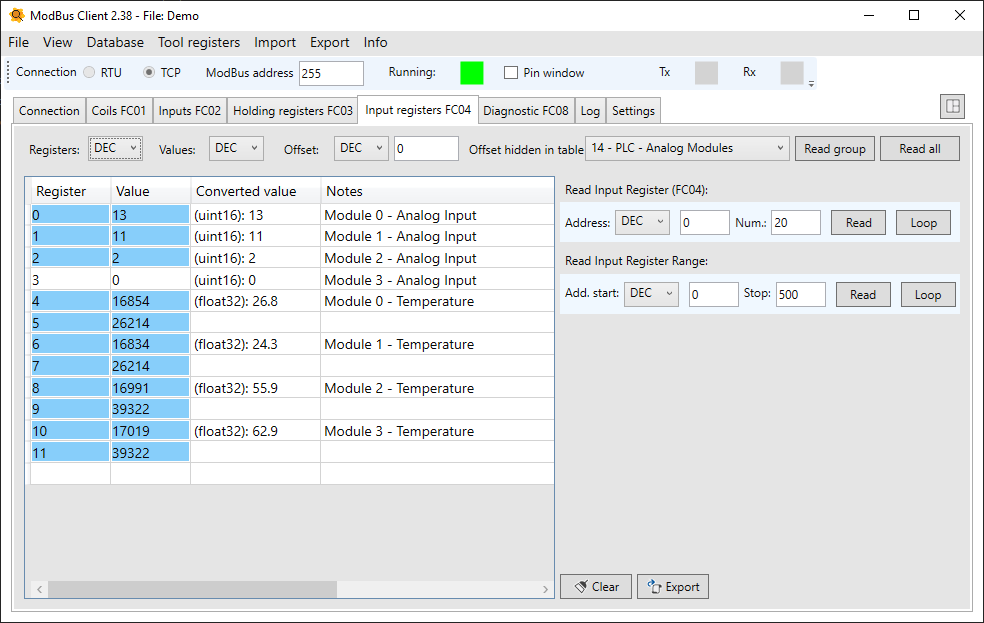
\includegraphics[width=0.75\textwidth]{../Img/ModBus_Client_Template_ReadDemo00.PNG}
\caption{}
\end{figure}

As shown in the previous image 32 bit values are casted using
two consecutive registers.